\documentclass[newpage]{homework}
\newcommand{\hwname}{Zooey Nguyen}
\newcommand{\hwemail}{zooeyn@ucla.edu}
\newcommand{\hwclass}{CS 146}
\newcommand{\hwtype}{Homework}
\newcommand{\hwnum}{4}
\usepackage{subfig}
\begin{document}
\maketitle


\question
For all plots, the accuracy is a bit lower at low k, peaking at a midrange k, and then decreasing again when k is high. This is expected as low k corresponds to overfitting and high k corresponds to underfitting. Whether the tiebreaker is one class or another does not significantly the trends of either graph, of course not affecting the odd k accuracies at all. This would make sense for a dataset where there are not many ties that need to be broken in the first place.
\begin{figure}[htbp]
    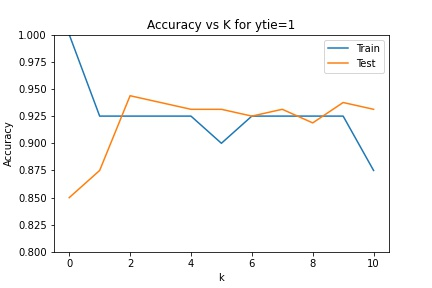
\includegraphics[width=0.5\textwidth]{1a.jpg}
    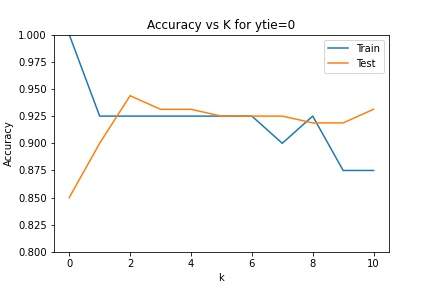
\includegraphics[width=0.5\textwidth]{1b.jpg}
\end{figure}


\question
The data does appear to be linearly separable.
\begin{figure}[htbp]
    \centering
    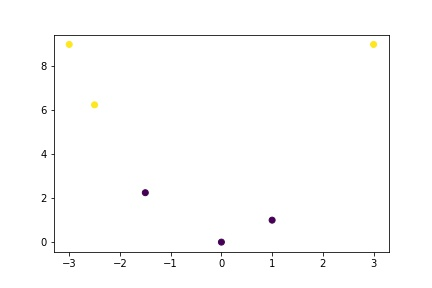
\includegraphics[width=0.5\textwidth]{2a.jpg}
\end{figure}

The two support vectors are the points (-2.5, 6.25) and (-1.5, 2.25). The separating line goes through the midpoint (-2, 4.25). The vector connecting them is in the direction (1, -4) so it has slope -4 for $x_2$ wrt $x_1$, which means the normal vector to the plane has the slope 1/4 for $x_2$ wrt $x_1$ and goes through the midpoint. Thus the equation of the line is $x_2 - 4.25 = \frac{1}{4} (x_1 + 2)$ so the equation of the plane is \fbox{$4x_2 + x_1 - 19 = 0$.}







\end{document}
